% -------------------------------------------------------------------
% APA-Style thesis LaTeX Template
% AUTHOR: Álvaro "Gondolindrim" Volpato (alvaro.volpato@usp.br)
% VERSION: 1.1
% PAGE: http://github.com/Gondolindrim/apaThesis
% LICENSE: Creative-Commons Non-commercial Share-Alike
%--------------------------------------------------------------------

% This is an example of document using the apaThesis class file,
% for a thesis that fits the American Phychology Association standards, described in 

% American Psychology Association (2009). Publication Manual of the American Psychological Association, sixth edition.

% It is supposed to be used as a template for a masters or PhD thesis. It was written in VIM and it contains
% folding data (the three "{") in the text. To enable this folding, type in vim:

% :setfoldmethod=marker

\documentclass{apaThesis}

% -----------------------------------------------
% (1) DOCUMENT DATA {{{1
% -----------------------------------------------

% Title and author
\title{APA Thesis LaTeX template}
\author{Álvaro Augusto Volpato}
\place{São Carlos, Brazil}
\writingdate{March 2019}
\affiliation{%
  University of São Paulo
  \par
  São Carlos School of Engineering
  \par
  Department of Electrical and Computer Engineering}
\advisor{Professor Dr. Luís Fernando Costa Alberto}
\preamble{Template document developed for thesis documents fulfilling the guidelines of the Publication Manual of the American Psychology Association, Sixth Edition}
%\renewcommand*\uniLogoWidth{0.2\textwidth}
\begin{document}

% PRINTING TITLE PAGE
\printtitlepage

% PRINTING FRONT MATTER
\printfrontmatter

% -----------------------------------------------
% (2) SECOND FRONT MATTER {{{1
% -----------------------------------------------

% SECOND FRONT MATTER IN SECOND LANGUAGE
% If this second frontmatter is not needed, comment lines 53-62.
% The anotherfrontmatter command takes seven arguments and prints a second frontmatter with them, without however changing the \title, \author, \place, \affiliation, \advisor keys which were defined previously.
% For its code, see line 544 of the class file apaThesis.cls .
\anotherfrontmatter
{Template de tese no estilo APA}%
{\theauthor}%
{São Carlos, Brasil}%
{Março de 2019}%
{Universidade de São Paulo \par %
Escola de Engenharia de São Carlos \par%
Departamento de Engenharia Elétrica e de Computação}%
{Professor Luís Fernando Costa Alberto}%
{Documento padronizado (``template'') desenvolvido para uso em teses segundo o Manual de Publicações da Associação Americana de Psicologia, Sexta Edição.}

% -----------------------------------------------
% (3) CATALOGRAPHIC CARD {{{1
% -----------------------------------------------

% CATALOGRAPHIC CARD
% I was not able to make a program for this as it can differ wildly between countries -- some won't even need one; therefore, unfortunately I was not able to make a macro or a custom command for this and it has to be edited manually. This is a widely used template, but please check if it fulfills the requirements of your institution and edit however needed.
\thispagestyle{empty}
\vspace*{\fill}
\begin{center}
\noindent\fbox{%
	\parbox{0.9\textwidth}{%
		\leftskip0.05\textwidth
		\vspace*{1cm}
		\parbox{0.8\textwidth}{%
		\ttfamily\footnotesize
		Volpato, Álvaro Augusto

		\begingroup\addtolength{\parindent}{2em}

			\thetitle\hphantom{ } / \theauthor; advisor Luís Fernando Costa Alberto - São Carlos 2019.			

			\thelastpage\hphantom{} p.\\

			Dissertation (Master's Degree - Graduate Program in Electrical Engineering) -- São Carlos School of Engineering, University of São Paulo - Brazil, 2019\\

			1. LaTeX. 2. American Psychology Association. I. Alberto, Luís Fernando Costa, advisor. II. Title.

		\endgroup
		\vspace*{1cm}
    }%
}
}
\end{center}

\cleardoublepage

% -----------------------------------------------
% (4) ABSTRACTS {{{1
% -----------------------------------------------
%\pagestyle{plain}

% In order to handle many abstracts in various languages, the "newabstract" environment was created, defined in lines 460-467 of the classe file "apaThesis.cls".
% Each time a new abstract is added, all that is needed is:
% \begin{newabstract}{<abstract name in that language>} 
% 	ABSTRACT CONTENT \\
% \noindent
% \textbf{<Keyword name in that language>}: keywords
% \end{newabstract}
% \newpage	

% (4.1) IN ENGLISH
\begin{newabstract}{Abstract}
	This is the abstract in english. \\
\noindent
\textbf{Keywords}: keyword 1, keyword 2, keyword 3 ...
\end{newabstract}

% (4.2) AUS DEUTSCH
\begin{newabstract}{Zusammenfassung}
Zusammenfassung aus Deutsch. \\

\noindent
\textbf{Stichwörter}: Stichwort 1, Stichwort 2,...
\end{newabstract}

% (4.3) EM PORTUGUÊS
\begin{newabstract}{Resumo}
	Resumo em português. \\
\noindent
\textbf{Palavras-chave}: palavra-chave 1, palavra-chave 2, ...
\end{newabstract}

% -----------------------------------------------
% (5) LISTS OF FIGURES, TABLES, SYMBOLS AND ACRONYMS {{{1
% -----------------------------------------------
% Figures and tables will be automatically added as they appear in text.

% LIST OF FIGURES
\listoffigures
\cleardoublepage

% LIST OF TABLES
\listoftables
\cleardoublepage

% -----------------------------------------------
% LIST OF ABBRV. AND SYMBOLS
% -----------------------------------------------
% This piece of code centralizes the LoA and LoS names, putting them in a HUGE and boldfaced font.
% I was not able to insert this inside a \newenvironment, because this snippet messes with the
% @makeschapter macro, which parameter #1 conflicts with the parameter number definition of the
% newenvironment giving a "Illegal number definition" error. 

\begingroup
	\makeatletter
		\def\chapter{\cleardoublepage\secdef\@chapter\@schapter}
		\def\@makeschapterhead#1{{\center\HUGE\sffamily\bfseries #1\par\nobreak\vskip 10\p@\vspace*{5mm} }}
	\makeatother

% The LoA and LoS can be removed by commenting their respective lines if not needed.
% Defining acronyms
\begin{acronyms}
	\acronym{OMIB}{One Machine Infinite Bus System}
	\acronym{CG}{Centralized Generation}
	\acronym{DG}{Distributed Generation}
	\acronym{RPGTs}{Renewable Power Generation Technologies}
	\acronym{MASs}{Multi-Agent Systems}
	\acronym{EPSs}{Electric Power Systems}
	\acronym{ESSs}{Energy Storage Systems}
	\acronym{MPPT}{Maximum Power Point Tracking}
	\acronym{PV}{Photovoltaic}
	\acronym{PBD}{Pinning-based Droop}
	\acronym{SM}{Synchronous Machine}
	\acronym{OAM}{One-Axis Model}
	\acronym{ICMPPT}{Incremental Conductance Maximum Power Point Tracking}
\end{acronyms}

\begin{listofsymbols}
	\item[$ \Gamma $] Gamma greek letter
	\item[$ \Lambda $] Lambda greek letter
	\item[$ \zeta $] Lowercase Zeta greek letter
	\item[$ \in $] Set theory belonging/contained in relation
	\item[$|\cdot|$] Complex absolute value
	\item[$\lVert \cdot \rVert$] Complex vector or matrix euclidian norm
\end{listofsymbols}

\endgroup

% -----------------------------------------------
% (6) TABLE OF CONTENTS {{{1
% -----------------------------------------------

\tableofcontents*
\cleardoublepage

% Redefine plain style
\pagestyle{fancy}

% -----------------------------------------------
% (7) EPIGRAPH {{{1
% -----------------------------------------------

\begin{newepigraph}
``An optimist will tell you the glass is half-full.
				
A pessimist will say it's half-empty.

An engineer will tell you the glass is twice the size it needs to be.''

\hfill --- Unknown Author
\end{newepigraph}

%% -----------------------------------------------
% (8) TEXT BODY {{{1
% -----------------------------------------------

% Begin page number at one and start arabic page numbering
\begintextbody

% ---------------------------------------------------------
\chapter{First steps: setting up your thesis}
% ---------------------------------------------------------

	\lettrine{T}{his} template is a joint effort between Álvaro Augusto Volpato --- graduate Electrical Engineering student from São Carlos School of Engineering (EESC) --- and Eduardo Graziozi Silva and Flavia Helena, from EESC's Library staff, to make an APA-style thesis template that abides to the formatting rules of the São Carlos School of Engineering at the University of São Paulo (EESC-USP). While Alvaro is the developer and maintainer, Eduardo and Flavia are the ones responsible for usage and distribution of the class throughout the University of São Paulo and specifically EESC. It is meant as a template for usage in thesis and dissertations written in English and Portuguese, although it can easily be translated to other languages and offers multi-language support.

	This template was written using the guidelines of the Publication Manual of the American Association of Psychology, Sixth Edition, which can be obtained at \href{https://apastyle.apa.org/manual/}{APA's official page}. The template example together with its documentation and files can be obtained and downloaded at \href{http://github.com/Gondolindrim/apaThesis}{its repository}. There you can clone the repository, fork it, submit pull requests and so on. This documentation is meant to offer guidelines to use this template: read it carefully to understand and use it how the author intended.

	To contact Álvaro for suggestions and feature requests, contact him at:

\begin{itemize}
	\item His e-mail \url{alvaro.volpato@usp.br};
	\item His GitHub page: \url{http://github.com/Gondolindrim}.
\end{itemize}

	This first chapter will show the first steps in setting yout document in this template: how the template works and how it is organized, how to to change basic features of the template, like page size, margins, fonts, how to set title, author, university name, abstracts and epigraph.

% ---------------------------------------------------------
	\section{How the template is organized}%{{{1
% ---------------------------------------------------------

	The template folder tree is organized in three basic folders, at the root folder, as depicted in figure \ref{fig:rootFolderTree}.

\begin{itemize}
	\item The {\ttfamily\small /images} folder stores all graphics and image-related files. These are included in the document through a special commend {\ttfamily\small \\includegraphics};
	\item The {\ttfamily\small /scripts} folder stores the codes, algorithms and listings that will be displayed in the thesis. These codes are displayed through a dedicated command {\ttfamily\small \\lstinputlisting}, which is used with a customized style defined in the class file;
	\item The {\ttfamily\small /tex} folder stores all TeX-related files, including the thesis text, the class file, appendixes.
\end{itemize}

\begin{figure}
\centering
\framebox[\textwidth]{%
\begin{minipage}{0.9\textwidth}
	\dirtree{%
	.1 /.
	.2 \textbf{/images}.	
	.2 \textbf{/scripts}.
	.2 \textbf{/tex}.
	}
\end{minipage}
}
\caption{Root folder folder tree.}\label{fig:rootFolderTree}
\end{figure}

	These settings can be changed anytime and even throughout the document (see sections \ref{sec:figures} and \ref{sec:scripts}); they were adopted as default in order to facilitate organizing data. It is recommended that the user keeps the folder tree intact in order to coherently add graphics and scripts to the document.

	The raw script of this template lies in the {\ttfamily\small tex} folder, as depicted in figure \ref{fig:texFolderTree}.

\begin{figure}
\centering
\framebox[\textwidth]{%
\begin{minipage}{0.9\textwidth}
	\dirtree{%
	.1 \textbf{/tex}.
		.2 apaThesis.cls .
		.2 main.tex .
		.2 refs.bib .
		.2 \textbf{/chapters} .
			.3 introduction.tex .
			.3 figs\_and\_tables.tex .
			.3 equations\_and\_math.tex .
			.3 references.tex .
		.2 \textbf{/appendixes} .
			.3 appendixA.tex .
			.3 appendixB.tex .
		.2 \textbf{/build} .
			.3 main.pdf .
			.3 Output files (*.toc, *.bbl, *.out et cetera) .
	}
\end{minipage}
}
\caption{{\ttfamily\small /tex} folder tree.}\label{fig:texFolderTree}
\end{figure}

	In the {\ttfamily\small /tex} folder tree,

\begin{itemize}
	\item {\ttfamily\small apaThesis.cls} is the TeX class file that stores the APA style guidelines and formats the document. It is invoked in the vey beggining of {\ttfamily\small main.tex}. It is recommended that this file is not edited nor moved/deleted unless needed;
	\item {\ttfamily\small main.tex} is the main LaTeX file and describes the organization and contents of the document. This is where the pre-textual elements (title, front matter, catalographic card, abstracts, lists of figures, tables, acronyms and symbols, table of contents) are set-up, invoked and built;
	\item {\ttfamily\small refs.bib} is the bibliography file, containing the references in BibTeX format;
	\item {\ttfamily\small /tex/chapters} folder contains the text contents of the chapters, each chapter separated into a single *.tex file. This is done so as to make editing easier; otherwise, all text content is added to a single main.tex file which becomes too big and harder to maintain, specially when using versioning softwares like Git;
	\item {\ttfamily\small /tex/appendixes} folder contains the appendixes text contents;
	\item {\ttfamily\small /tex/build} folder contains the final build files, including the *.pdf file generated and other build files. It is recommended that the build folder be separated because those output files can flood the file tree and difficult maintenance.
\end{itemize}

% ---------------------------------------------------------
	\section{Changing page geometry}%{{{1
% ---------------------------------------------------------

	The default implementation of the example uses the US Letter Paper size with 1 inch margins, as recommended by APA in their Publication Manual. This is done in the first lines of the {\ttfamily\small main.tex} file, by calling the class file with no options, as in listing \ref{lst:usLetter}.

\begin{lstlisting}[caption = {Using the class with US Letter paper size}, label = {lst:usLetter}, style = prettyListing, language = tex]
\documentclass{apaThesis}
\end{lstlisting}

	There is also an option for A4 paper, by invoking the {\ttfamily\small a4paper} option as in listing \ref{lst:a4paper}.

\begin{lstlisting}[caption = {Using the class with A4 paper size}, label = {lst:a4paper}, style = prettyListing, language = tex]
\documentclass[a4paper]{apaThesis}
\end{lstlisting}

	These two sizes should cover most universities requirements. If however a custom size needs to be used, you can declare a custom size in the first section of the class file, you can comment line 67 of the class file, uncomment line 70 and use the {\ttfamily\small paperwidth} and {\ttfamily\small paperheight} options, editing the height and width options as desired. You can also alter margin values if needed.

% ---------------------------------------------------------
	\section{Changing fonts used}%{{{1
% ---------------------------------------------------------

	The fonts definitions of the class lie in lines 81-90 of the class file, in the {\ttfamily\small (2) MAIN FONTS}. Any of the used fonts can be changed by the user; for a list of LaTeX supported fonts, see the \href{https://tug.org/FontCatalogue/}{\LaTeX\ font Catalogue}.

\begin{itemize}
	\item Font Rosario is used as the sans serif for titles and some highlights. This font is called by using the command {\ttfamily \textbackslash usepackage\{Rosario\}};
	\item Font Times New Roman is used as serif font for most of the text body. This font is called by the {\ttfamily\small \textbackslash usepackage\{times\}}. Times font is also used as the main math font by using {\ttfamily\small \textbackslash usepackage\{newtxmath\}}
	\item Font Inconsolata is used as the monospace font. This font is called by the {\ttfamily\small \textbackslash usepackage\{inconsolata\}}.
	\item {\ttfamily\small \textbackslash usepackage\{lettrine\}} is used to display a big letter at the beggining of every chapter.
\end{itemize}

% ---------------------------------------------------------
	\section{How to build the main.tex file}%{{{1
% ---------------------------------------------------------

	Two things must be noted when building the files: the first, that the build folder must be specified (otherwise the output files will be generated at the {\ttfamily\small /tex} folder, flooding it) and that the PDFLaTeX engine must be used (neither XeLaTex nor LuaLaTeX will work).

	\subsection{In a command-line}

	In Linux and Windows' command prompt, when using the shell script, building the main file is done by using the following command in the {\ttfamily\small /tex} folder:

\begin{center} {\ttfamily\small pdflatex --output-directory=build main.tex} \end{center}

	If you need to invoke PDFLaTeX from the root folder, use:

\begin{center} {\ttfamily\small pdflatex --output-directory=./tex/build ./tex/main.tex} \end{center}

	\subsection{In a dedicated TeX editor}

	If an editor like TeXMaker, Lyx or TeXStudio is used, these parameters (using PDFLaTeX and the build directory) must be set expressly in the editor configurations. If Overleaf/ShareLaTeX is used, then this configuration is not needed as the platform generates output in real-time and the PDF file can be downloaded at any time.

% ---------------------------------------------------------
	\section{Setting up university logo, thesis title, front matter and abstracts}%{{{1
% ---------------------------------------------------------

	After setting up the basic geometry of the document, and before inputting the text body, you should input your name, thesis title, advisor name, university logo and name, and so on. This section will go through a step-by-step way to do this.

	\subsection{Change basic metadata: title, names and university logo}

	First, go to the first section of {\ttfamily\small main.tex} called {\ttfamily\small ``(1) DOCUMENT DATA''} and edit the data accordingly. Beware that the preamble text must generally follow a convention by your university or institute, so be sure to check past thesis and use the same format. Also be sure to correctly write the affiliation out; generally, the first line is the university name, second line is the institute name and third line is the department or research group name.

	The university logo can be changed by simply replacing the {\ttfamily\small ./images/uniLogo.pdf} file with your university's or institute's logo. You might need to adjust this logo size by adjusting the {\ttfamily\small \textbackslash uniLogoWidth} command in line 38 of {\ttfamily\small main.pdf}. The default value is {\ttfamily\small 0.2\textbackslash textwidth}.

% ---------------------------------------------------------
	\subsection{Second front matter}%{{{2
% ---------------------------------------------------------
	
	Many universities will require that after the english front matter, a second front matter is added in the native language of that institute or university. This is done by editing the parameters in lines 55-64 of {\ttfamily\small main.pdf}. If you don't need a second frontmatter, commend out these lines.

% ---------------------------------------------------------
	\subsection{Catalographic card}%{{{2
% ---------------------------------------------------------

	The catalographic card is a piece of meta data used by libraries to classify and organized their stored works. Generally they follow a very similar structure throughout the world.

	As I was not able to automatize this card, it is needed that you edit it accordingly to the structure your university requires. The example pattern is used throughout the world and should be very common; all you need is to change the names accordingly.

% ---------------------------------------------------------
	\subsection{Abstracts}%{{{2
% ---------------------------------------------------------

	Adding an abstract is easily done through the {\ttfamily\small newabstract} environment. This environment is defined in the class file so that you can add as many abstracts as you wish, in as many languages.

	To add a new abstract in english, use the following code:

\begin{lstlisting}[caption = {Adding an abstract in english}, label = {lst:englishAbstract}, style = prettyListing, language = tex]
\begin{newabstract}{Abstract}
	This is the abstract in english. \\
\noindent
\textbf{Keywords}: keyword 1, keyword 2, keyword 3 ...
\end{newabstract}
\end{lstlisting}

	To add an abstract in another language, use the other language names and abstract body; for example, to add an abstract in german, use:

\begin{lstlisting}[caption = {Adding an abstract in german}, label = {lst:germanAbstract}, style = prettyListing, language = tex]
\begin{newabstract}{Zusammenfassung}
Zusammenfassung aus Deutsch. \\
\noindent
\textbf{Stichw\"{o}rter}: Stichwort 1, Stichwort 2,...
\end{newabstract}
\end{lstlisting}
	
	Beware that in most universities the english abstract will be needed, and an abstract in another language is optional. Either case, at least an abstract should be devised.

	\subsubsection{Modifying abstract properties} %---------------------------------------------

		The {\ttfamily\small newabstract} environment is defined in section {\ttfamily\small ``(13) NEWABSTRACT ENVIRONMENT''} of the class file. The default implementation is accepted widely and will most probably fit your university's requirements, but can be changed as desired.

% ---------------------------------------------------------
	\subsection{Acronyms and symbols}%{{{2
% ---------------------------------------------------------

	Next are the lists of acronyms and symbols. The example shows how to add acronyms:

\begin{lstlisting}[caption = {Adding an acronym}, label = {lst:addingAcronym}, style = prettyListing, language = tex]
	%\acronym{<acronym>}{<What the acroym means>}
	\acronym{SG}{Synchronous Generator}
\end{lstlisting}

	The procedure is the same for symbols:

\begin{lstlisting}[caption = {Adding an acronym}, label = {lst:addingAcronym}, style = prettyListing, language = tex]
	%\item{<symbol>}{<What the symbol means>}
	\item{$k_B$}{Boltzmann's constant}
\end{lstlisting}

	Also note that the {\ttfamily\small <symbol>} key can be a math expression, in between {\ttfamily\small \$} characters (the example document contains examples like this).

	If acronyms and/or symbols are not needed, you can comment or delete the {\ttfamily\small acronyms} (lines 170-184 in the {\ttfamily\small main.tex} document) and {\ttfamily\small listofsymbols} (lines 186-193 in the {\ttfamily\small main.tex} document) environments.

% ---------------------------------------------------------
	\subsection{Epigraph}%{{{2
% ---------------------------------------------------------

	The epigraph is that little sentence or thought you add in italics, generally in latin, with the sole purpose of sounding smart.

	To add an epigraph, use the {\ttfamily\small newepigraph} environment as used in line 211 of {\ttfamily\small main.tex}. If you don't want to sound smart, you can comment the environment (lines 211-219).

% ---------------------------------------------------------
	\subsection{First compile and adding packages}%{{{2
% ---------------------------------------------------------

	This is the end of the initial setting up steps. You should be able to compile your document now -- albeit with no text -- and see if it meets your requirements. The next chapter will focus on how to add text body.

	In order to add your packages to the document, use the {\ttfamily\small \textbackslash usepackage[...]\{...\}} commands before the {\ttfamily\small \textbackslash begin\{document\}} command, ideally right below {\ttfamily\small \textbackslash documentclass\{apaThesis\}}.

% ---------------------------------------------------------
	\section{Adding text chapters and appendixes}%{{1
% ---------------------------------------------------------

	The text body can be added as a normal \LaTeX\ text.

	The main example uses the {\ttfamily\small \textbackslash input} command, which allows you to input text from another file into your {\ttfamily\small main.pdf} file. This allows you to write each piece of text in a dedicated file, making maintenance easier. If a single {\ttfamily\small main.pdf} is used for the whole document, it can grow too big and make version management difficult, specially with Git, by generating conflicts between commits.

	The figure, table and listing labels are kept throughout the whole document even if they are defined in different files; for example, say that in {\ttfamily\small chapter3.tex} you defined a figure with label {\ttfamily\small fig:graph}. You can call this same label in {\ttfamily\small chapter2.tex} just as if the chapters were written in the same file and not in separate files. For example, figure \ref{fig:ivCurve} is defined in the {\ttfamily\small /tex/appendixes/appendixA.tex} while this introduction chapter file is {\ttfamily\small /tex/chapters/introduction.tex} and the figure label can be used by typing {\ttfamily\small \textbackslash ref\{fig:ivCurve\}}, which is how its label is defined in the appendix file.

	To add chapters and text body, use the syntax in listing \ref{lst:addingChapter}. Add that command after the {\ttfamily\small /begintextbody} command and between {\ttfamily\small \textbackslash bibliography}.

\begin{lstlisting}[caption = {Adding a chapter to text body}, label = {lst:addingChapter}, style = prettyListing, language = tex]
	%\input{<Chapter *.tex file>}
	\input{./chapters/chapter1.tex}
\end{lstlisting}

	Note that the chapter files do not need headings or packages, as all configuration is inherited by them from {\texttt\small main.pdf}. By default in the template, chapter files are added to the {\ttfamily\small /tex/chapters} folder, but you can create further folders and add them to your {\ttfamily\small input} command.

	This process is the same for adding appendixes; however, those should be added after the {\ttfamily\small \textbackslash appendix} command, since this command makes appendixes be numbered in progressive letters (Appendix A, Appendix B \textit{et cetera}).


% ----------------------------------------------
\chapter{Figures and tables}
% ----------------------------------------------

	This chapter verses on how to add figures, tables and scripts to your document.

	Adding those features is pretty straightforward as they are already formatted to the APA style. The only thing you should take care when adding these elements is the element size in relation to the page, that is, if the figure or table does not extend past the margins.

	For figures, this is generally a tradeoff between having legible text in the figure and having enough page space, meaning that you should adjust the image until it is readable and legible and its size is correct.

% ----------------------------------------------
	\section{Adding figures}
% ----------------------------------------------

	To add a figure to the document, use syntax in listing \ref{lst:addingFigure}.

\begin{lstlisting}[caption = {Basic code for adding a figure.}, label = {lst:addingFigure}, style = prettyListing, language = tex]
\begin{figure}[h]
	\centering
	\includegraphics[<Scaling and angle options>]{<Figure file location>}
	\caption{<Figure caption>}
	\label{<Human-readable label>}
\end{figure}
\end{lstlisting}

	{\ttfamily\small \textbackslash centering } forces figure centering; {\ttfamily\small \textbackslash caption\{\} } is the figure caption that explains or defines it; {\ttfamily\small \textbackslash label\{\} } is the human-readable label that you use to reference the image in the text.

	The command {\ttfamily\small \textbackslash includegraphics[]\{\} } is the command to insert the figure. This command defines the size of the inserted image; for example, using {\ttfamily\small \textbackslash width = 5cm} will add a five-centimeter-wide figure that is also vertically scaled. See listing \ref{lst:5cmEESC}; figure \ref{fig:5cmEESC} shows the output of that code.

\begin{lstlisting}[caption = {5cm-wide EESC logo (figure \ref{fig:5cmEESC}).}, label = {lst:5cmEESC}, style = prettyListing, language = tex]
\begin{figure}[h]
	\centering
	
\includegraphics[width = 5cm]{../images/uniLogo.pdf}
	\caption{Centimeter-wide EESC logo}
	\label{fig:5cmEESC}
\end{figure}
\end{lstlisting}

\begin{figure}[h]
	\centering
	
\includegraphics[width = 5cm]{../images/uniLogo.pdf}
	\caption{Five-centimeter-wide EESC logo.}
	\label{fig:5cmEESC}
\end{figure}

	This procedure is highly customizable, according to the parameters of the various environments and commands used.

	\subsection{Figure placement}

	 The {\ttfamily\small figure} environment makes a floating figure that is adjusted by the \LaTeX\ engine . The {\ttfamily\small [h]} option defines that the figure should be placed preferably where it is placed in the source text, but that does not mean it will necessarily be placed there. For more placing options, see \href{https://tex.stackexchange.com/questions/35125/how-to-use-the-placement-options-t-h-with-figures}{this StackExchange page}. There are also other options, like:

\begin{itemize}
	\item The {\ttfamily\small [t]} option will position the figure at the top of the page;
	\item The {\ttfamily\small [b]} option will position the figure at the bottom of the page;
	\item The {\ttfamily\small [p]} option will position the figure at a special page reserved for floating environments only;
	\item The {\ttfamily\small [H]} option forces the engine to place the figure at \textit{exactly} the location it was defined in the source file.
\end{itemize}

% ----------------------------------------------
	\subsection{Scaling figures}
% ----------------------------------------------

	The  {\ttfamily\small \textbackslash includegraphics} command has a variety of options, like {\ttfamily\small width} and {\ttfamily\small height}, used too adjust the width and height of the image; if only one is used, the image is scaled to that dimension. For example, in listing \ref{lst:5cmEESC} only the width option was used, so the image height was scaled so that the width would be the specified value. If, however, both height and width values are specified, the image will be adjusted for the given values. Listing \ref{lst:53cmEESC} shows an example of both values given and image \ref{fig:53cmEESC} shows the result. Note that the image looks flattened because the height and width values given are not proportional to the original proportions of the image.

\begin{lstlisting}[caption = {5cm-wide EESC logo (figure \ref{fig:53cmEESC}}), label = {lst:53cmEESC}, style = prettyListing, language = tex]
\begin{figure}[h]
	\centering
	
\includegraphics[width = 5cm, height = 3cm]{../images/uniLogo.pdf}
	\caption{Five centimeter wide, three centimeter tall EESC logo}
	\label{fig:53cmEESC}
\end{figure}
\end{lstlisting}

\begin{figure}[h]
	\centering
	
\includegraphics[width = 5cm, height = 3cm]{../images/uniLogo.pdf}
	\caption{Five centimeter wide, three centimeter tall EESC logo}
	\label{fig:53cmEESC}
\end{figure}

	To make it easier for you to scale graphics in relation to the text column width, this length is given in \LaTeX\ by the command {\ttfamily\small \textbackslash textwidth}; for instance, to insert an image that has width of a quarter the text width, use {\ttfamily\small width = 0.25\textbackslash textwidth}, as in listing \ref{lst:quarterTextEESC}. Figure \ref{fig:quarterTextEESC} shows the output of such code. Giving height and width values in fractions of the text column width guarantees that the image will look more organic and better placed.

\begin{lstlisting}[caption = {EESC logo with quarter the text column width (figure \ref{fig:quarterTextEESC}}), label = {lst:quarterTextEESC}, style = prettyListing, language = tex]
\begin{figure}[h]
	\centering
	
\includegraphics[width = 0.25\textwidth]{../images/uniLogo.pdf}
	\caption{EESC logo with a quarter the text column width}
	\label{fig:quarterTextEESC}
\end{figure}
\end{lstlisting}

\begin{figure}[h]
	\centering
	
\includegraphics[width = 0.25\textwidth]{../images/uniLogo.pdf}
	\caption{EESC logo with a quarter the text column width.}
	\label{fig:quarterTextEESC}
\end{figure}

% ----------------------------------------------
	\subsection{Rotating figures}
% ----------------------------------------------

	The  {\ttfamily\small \textbackslash includegraphics} command also has an {\ttfamily angle} option which rotates the image by a given angle, measured in degrees. Listing \ref{lst:45degreeEESC} shows a 45-degree rotated logo, and figure \ref{fig:45degreeEESC} shows the results.

\begin{lstlisting}[caption = {EESC logo rotated 45 degrees (figure \ref{fig:45degreeEESC}}), label = {lst:45degreeEESC}, style = prettyListing, language = tex]
\begin{figure}[h]
	\centering
	
\includegraphics[width = 3cm, angle = 45]{../images/uniLogo.pdf}
	\caption{EESC logo rotated by 45 degrees.}
	\label{fig:45degreeEESC}
\end{figure}
\end{lstlisting}

\begin{figure}[h]
	\centering
	
\includegraphics[width = 3cm, angle = 45]{../images/uniLogo.pdf}
	\caption{EESC logo rotated 45 degrees.}
	\label{fig:45degreeEESC}
\end{figure}

% ----------------------------------------------
	\section{Adding tables}
% ----------------------------------------------

	Tables are a straightforward way to display data. The APA Publication Manual does recommend a particular table format, which is achieved by the code in listing \ref{lst:basicTable}. The {\ttfamily table} environment is pretty much alike the figure one in that it takes the same alignment options, caption and label convention. So all alignment options for the figures apply here, as well as caption and label.

\begin{itemize}
	\item The {\ttfamily table} environment sets a floating type for the table which positioning parameters are the same as figures;
	\item The {\ttfamily tabular} environment effectively code the table;
	\item The {\ttfamily <Column alignment options>} are passed to the tabular environment to define how many columns a table has and each columns alignment option;
	\item The {\ttfamily hline} command prints a horizontal line in the table spanning all of its width;
	\item The {\ttfamily \textbackslash caption} command defines the table caption;
	\item The {\ttfamily \textbackslash label} command defines a human-readable label by which the table can be referenced in the text.
\end{itemize}

\begin{lstlisting}[caption = {Basic table code}, label = {lst:basicTable}, style = prettyListing, language = tex]
\begin{table}[h]
	\begin{center}
		\begin{tabular}{<Column alignment options>}
			\hline
			<Header code> \\
			\hline
			<Rows code>\\
			\hline
		\end{tabular}
		\caption{<Table caption>}
		\label{<Human-readable label>}
	\end{center}
\end{table}
\end{lstlisting}

% ----------------------------------------------
		\subsection{Coding your table}
% ----------------------------------------------

	Table coding is fairly simple, with a basic rule: cells are separeted by a {\ttfamily \&} character and rows are broken using a double backslash sequence \textbackslash \textbackslash. Table \ref{tab:exampleTable} shows an example table used to exemplify table coding; this table has three columns with the first one left-aligned and the other ones center-aligned.

	Before inserting table data, is it important to input first the number of columns the table will have and the alignment of each column. This is done by passing the alignment options to the {\ttfamily tabular} environment.

	Each column can be centered ({\ttfamily c}), left aligned ({\ttfamily l}) or right aligned ({\ttfamily r}). In the example table of listing \ref{tab:exampleTable}, this is done by passing the {\ttfamily \{l c c\}} option, which defines the table will have three columns and each columns alignment.

	According to the APA Publication Manual, tables should have boldface headers. The header row should be separated by a horizontal line, at its top and bottom. Boldface is achieved by the {\ttfamily \textbackslash textbf\{\}} command and the horizontal line is achieved by the {\ttfamily hline} command.

\begin{lstlisting}[caption = {Example table (table \ref{tab:exampleTable})}, label = {lst:exampleTable}, style = prettyListing, language = tex]
\begin{table}[h]
	\begin{center}
		\begin{tabular}{l c c}
			\textbf{Name} & \textbf{Age} & \textbf{Height} (m) \\
			\hline
			John & 25 & 1.80\\
			Mary & 34 & 1.72\\
			Janett & 14 & 1.54\\
			\hline
		\end{tabular}
		\caption{Age and height example table.}
		\label{tab:exampleTable}
	\end{center}
\end{table}
\end{lstlisting}

\begin{table}[h]
	\begin{center}
		\begin{tabular}{l c c}
			\hline
			\textbf{Name} & \textbf{Age} & \textbf{Height} (m) \\
			\hline
			John & 25 & 1.80\\
			Mary & 34 & 1.72\\
			Janett & 14 & 1.54\\
			\hline
		\end{tabular}
		\caption{Age and height example table.}
		\label{tab:exampleTable}
	\end{center}
\end{table}

	First of all


%% ----------------------------------------------
% (9) BIBLIOGRAPHY {{{1
% -----------------------------------------------
\bibliography{refs}

% -----------------------------------------------
% (10) APPENDIXES {{{1
% -----------------------------------------------

\part*{Appendixes}
\appendix

\chapter{PV Panel Curves and simulation program} \label{ap:pvPanelCurves}

	This appendix shows the simulation curves of the photovoltaic panel static equation \eqref{eq:PVPanelModelModified}. It also shows listing \ref{lst:pvPanelCurves}, the Python program used to obtain those curves. The parameter values of the photovoltaic panels are denoted in table \ref{tab:panelParameters}.

\begin{figure}[h]
	\centering
	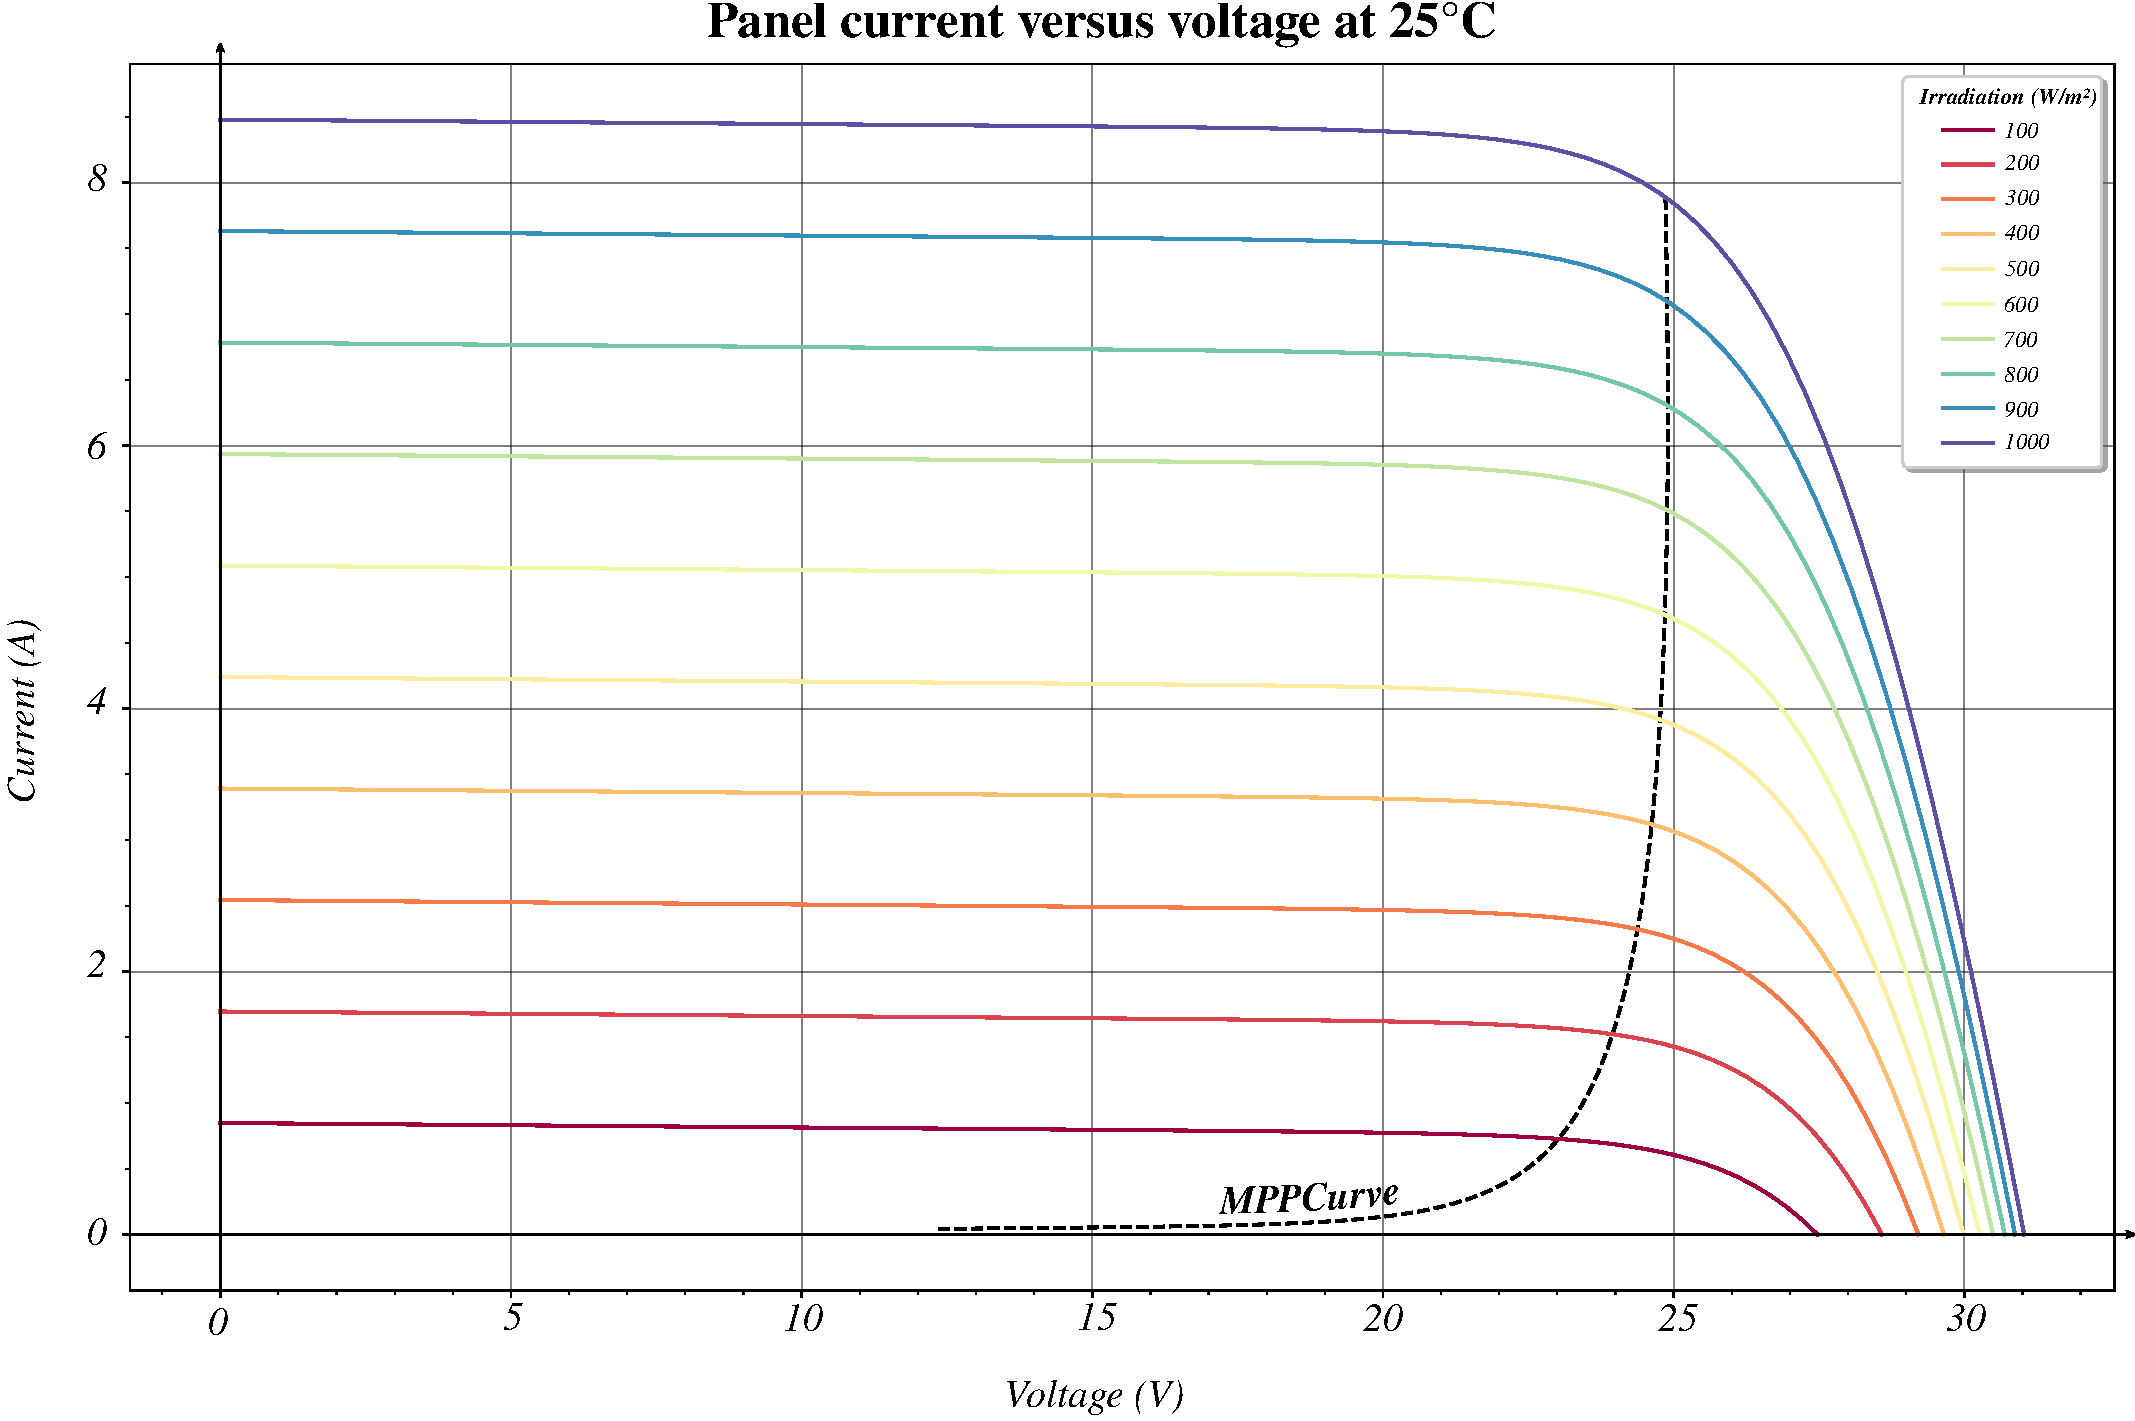
\includegraphics[angle = -90, width = 0.9\textwidth]{../images/pvPanelCurves/ivCurve.pdf}
	\caption{Panel transconductance (continuous) and MPP (dashed) curves with fixed temperature $\theta_{SRC}$ and varying irradiance.}
	\label{fig:ivCurve}
\end{figure}

	\lstinputlisting[caption = {Python PV panel simulation program developed to generate figures \ref{fig:ivCurve} to \ref{fig:pvCurveVaryingTemperature}}, label = {lst:pvPanelCurves}, style = prettyListing, language = Python]{../images/pvPanelCurves/mppTracking.py}

\chapter{Second appendix} \label{ap:ap2}

	This is the second appendix.


\end{document}
